% =============================================================================
% CHAPTER THREE - MATERIALS AND METHODS
%
% STATUS: stub. Holds the system-specific figures moved out of Chapter One,
% where they did not belong. Chapter One takes general, conceptual figures;
% architecture diagrams, hardware layouts and protocol chains belong here.
%
% Section skeleton follows Appendix III A of the UB guide:
%   3.1 The methodology            3.5 Treatment and analysis of the data
%   3.2 Specific procedures        3.6 Ethical considerations
%   3.3 Research population/sample 3.7 Scope of the current research
%   3.4 Instrumentation
%
% Source material: project fin update with reviewers/main_article.tex,
% sections 3 (System and Architecture) and 4 (Materials and Methods).
%
% NOT YET INCLUDED in main.tex. Enable the \include line once Chapter Two
% exists, so the built document does not jump from Chapter One to Chapter
% Three.
% =============================================================================

\chapter{Materials and Methods}
\label{ch:methods}

\section{The Methodology}
\label{sec:methodology}

%% TODO: research design, from the article's Materials and Methods section.

\section{Specific Procedures}
\label{sec:procedures}

\subsection{Overall System Architecture}
\label{subsec:architecture}

The system is organised into five tiers with explicit interfaces between them,
shown in Figure~\ref{fig:five-tier}. Sensing, gateway processing, mesh
networking, distributed ledger and application services are separated so that
each tier can be characterised and its cost measured independently.

\begin{figure}[htbp]
  \centering
  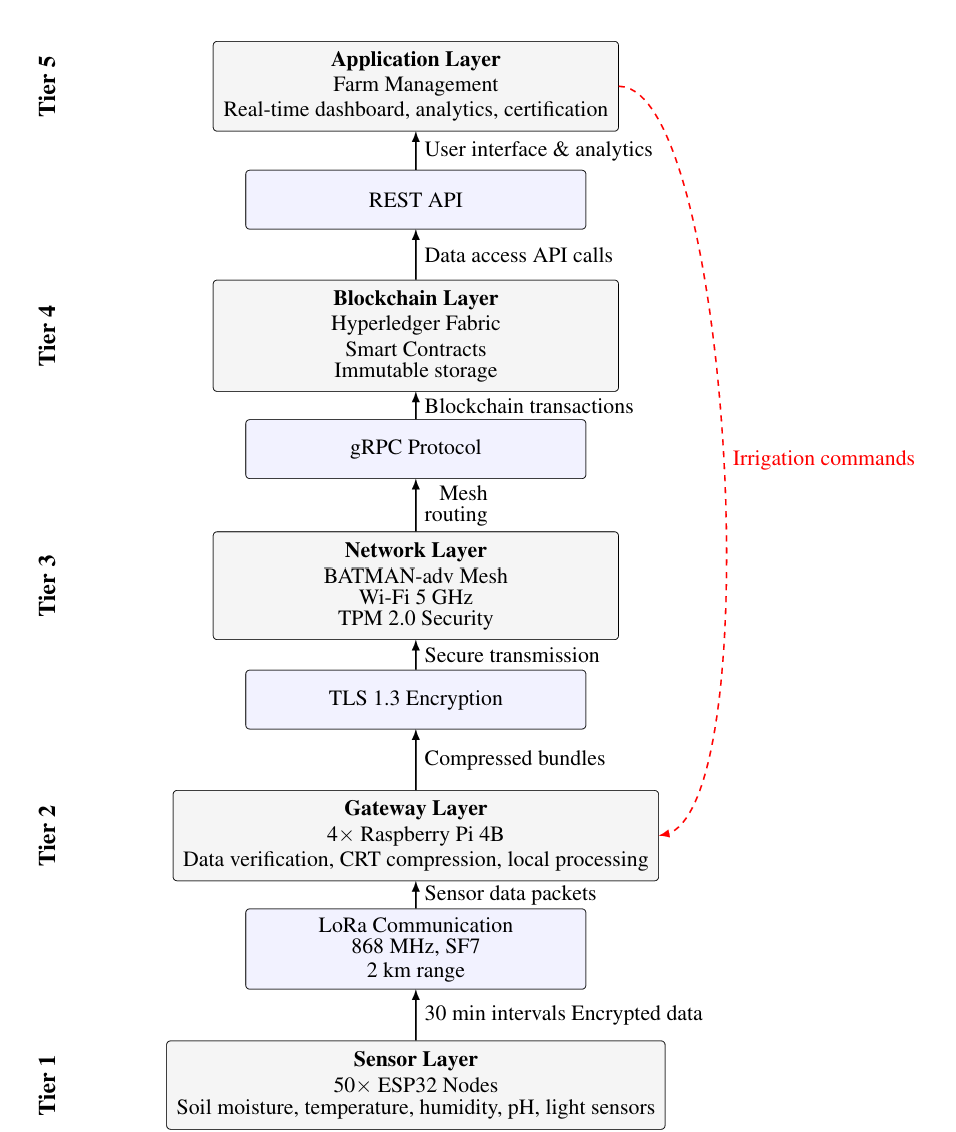
\includegraphics[width=0.72\textwidth]{figures/five-tier-architecture.png}
  \caption{Five-tier organisation of the agricultural data processing system,
           from \gls{esp32} sensing nodes through \gls{lora} uplink, gateway
           processing and the permissioned ledger to farm management
           analytics.}
  \label{fig:five-tier}
\end{figure}

\subsection{End-to-End Data Path}
\label{subsec:datapath}

Figure~\ref{fig:crt-pipeline} traces a single reading through the pipeline,
from analogue acquisition and residue encoding at the node, through
reconstruction by Garner's algorithm and signature verification at the
gateway, to on-chain anchoring and irrigation actuation.

\begin{figure}[htbp]
  \centering
  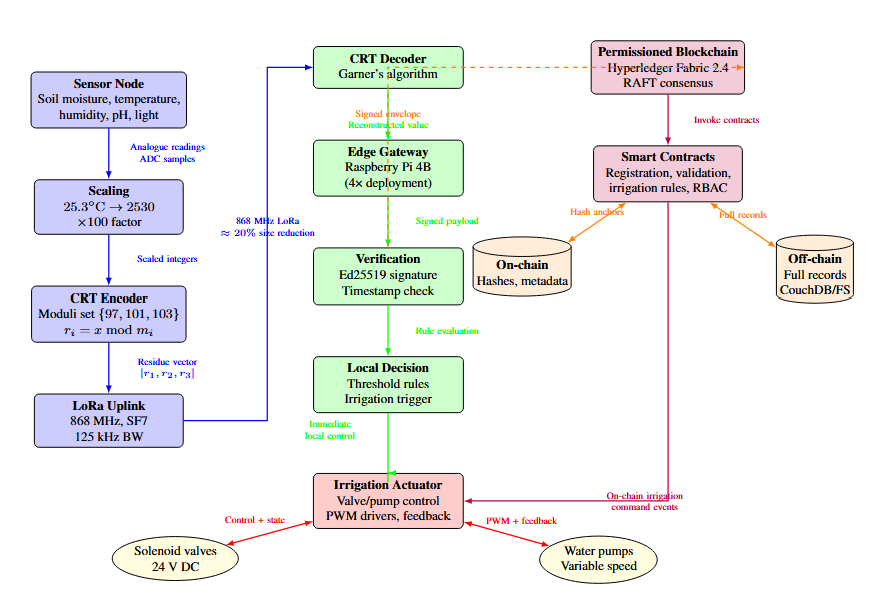
\includegraphics[width=\textwidth]{figures/crt-pipeline.png}
  \caption{End-to-end path of a single sensor reading. Residue encoding at the
           node (left) and reconstruction at the gateway (centre) bracket the
           transmission, while the permissioned ledger (right) anchors hashes
           on chain and retains full records off chain.}
  \label{fig:crt-pipeline}
\end{figure}

\subsection{Identity and Credential Enrolment}
\label{subsec:enrolment}

Figure~\ref{fig:identity} shows the enrolment chain. A root \gls{ca} issues
credentials to an enrolment authority, which issues gateway certificates and,
in turn, per-region sensor certificates.

\begin{figure}[htbp]
  \centering
  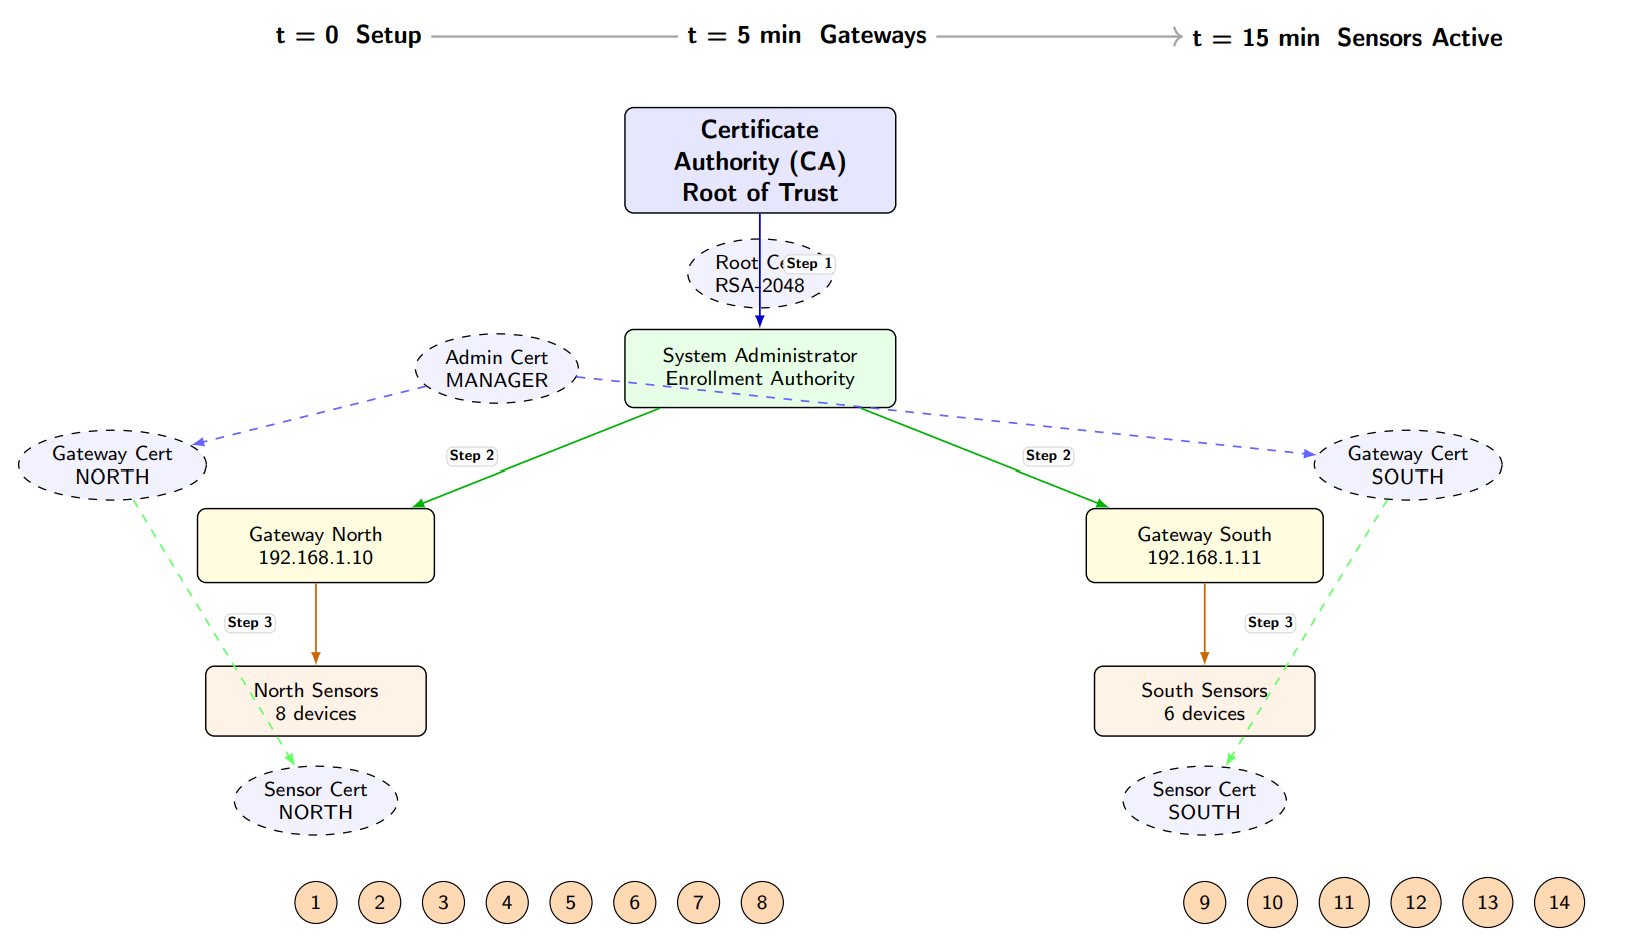
\includegraphics[width=0.92\textwidth]{figures/identity-enrolment.png}
  \caption{Certificate enrolment chain from the root \gls{ca} through the
           enrolment authority to gateway and sensor credentials.}
  \label{fig:identity}
\end{figure}

\section{Research Population or Sample}
\label{sec:population}

%% TODO: 50 ESP32 nodes, 4 Raspberry Pi 4B gateways, deployment site.

\section{Instrumentation}
\label{sec:instrumentation}

%% TODO: hardware design, sensor calibration, pilot study, data collection.

\section{Treatment and Analysis of the Data}
\label{sec:analysis}

%% TODO: metrics, statistical treatment, M/D/1 model.

\section{Ethical Considerations}
\label{sec:ethics}

%% TODO: data ownership, farmer consent, commercial confidentiality.

\section{Scope of the Current Research}
\label{sec:methods_scope}

%% TODO: boundary of what was implemented and measured.
